\documentclass[14pt]{extbook}
\usepackage{multicol, enumerate, enumitem, hyperref, color, soul, setspace, parskip, fancyhdr} %General Packages
\usepackage{amssymb, amsthm, amsmath, latexsym, units, mathtools} %Math Packages
\everymath{\displaystyle} %All math in Display Style
% Packages with additional options
\usepackage[headsep=0.5cm,headheight=12pt, left=1 in,right= 1 in,top= 1 in,bottom= 1 in]{geometry}
\usepackage[usenames,dvipsnames]{xcolor}
\usepackage{dashrule}  % Package to use the command below to create lines between items
\newcommand{\litem}[1]{\item#1\hspace*{-1cm}\rule{\textwidth}{0.4pt}}
\pagestyle{fancy}
\lhead{Progress Quiz 2}
\chead{}
\rhead{Version B}
\lfoot{4389-3341}
\cfoot{}
\rfoot{Summer C 2021}
\begin{document}

\begin{enumerate}
\litem{
Find the equation of the line described below. Write the linear equation in the form $ y=mx+b $ and choose the intervals that contain $m$ and $b$.\[ \text{Perpendicular to } 7 x + 8 y = 6 \text{ and passing through the point } (10, 8). \]\begin{enumerate}[label=\Alph*.]
\item \( m \in [0.99, 1.5] \hspace*{3mm} b \in [-2, 1] \)
\item \( m \in [0.06, 0.99] \hspace*{3mm} b \in [-4.43, -2.43] \)
\item \( m \in [0.99, 1.5] \hspace*{3mm} b \in [-4.43, -2.43] \)
\item \( m \in [-1.64, -0.82] \hspace*{3mm} b \in [13.43, 23.43] \)
\item \( m \in [0.99, 1.5] \hspace*{3mm} b \in [1.43, 4.43] \)

\end{enumerate} }
\litem{
Solve the equation below. Then, choose the interval that contains the solution.\[ -6(15x + 17) = -3(-19x + 18) \]\begin{enumerate}[label=\Alph*.]
\item \( x \in [-5.08, -4.19] \)
\item \( x \in [-0.63, 0.17] \)
\item \( x \in [0.24, 1.68] \)
\item \( x \in [-1.11, -0.91] \)
\item \( \text{There are no real solutions.} \)

\end{enumerate} }
\litem{
Solve the equation below. Then, choose the interval that contains the solution.\[ -11(-3x + 17) = -7(4x -14) \]\begin{enumerate}[label=\Alph*.]
\item \( x \in [-3.1, 0] \)
\item \( x \in [3.8, 6.6] \)
\item \( x \in [0.6, 2.7] \)
\item \( x \in [16.2, 18.7] \)
\item \( \text{There are no real solutions.} \)

\end{enumerate} }
\litem{
Write the equation of the line in the graph below in Standard Form $Ax+By=C$. Then, choose the intervals that contain $A, B, \text{ and } C$.
\begin{center}
    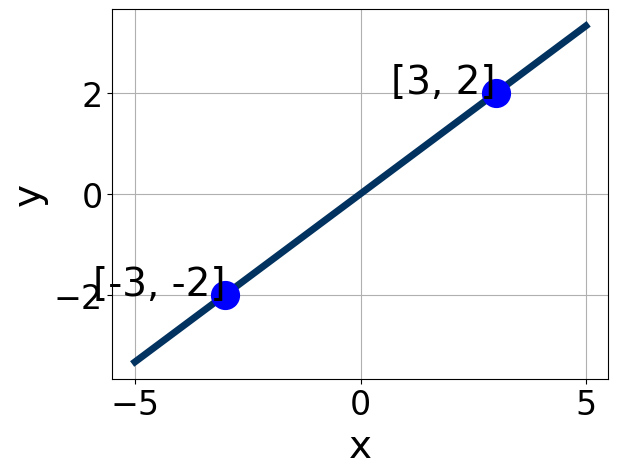
\includegraphics[width=0.5\textwidth]{../Figures/linearGraphToStandardCopyB.png}
\end{center}
\begin{enumerate}[label=\Alph*.]
\item \( A \in [-1.1, -0.5], \hspace{3mm} B \in [0.97, 1.03], \text{ and } \hspace{3mm} C \in [-1, 1] \)
\item \( A \in [-1.1, -0.5], \hspace{3mm} B \in [-2.47, -0.95], \text{ and } \hspace{3mm} C \in [-1, 1] \)
\item \( A \in [-4.3, -0.7], \hspace{3mm} B \in [1.95, 3.12], \text{ and } \hspace{3mm} C \in [-1, 1] \)
\item \( A \in [1.4, 2.8], \hspace{3mm} B \in [1.95, 3.12], \text{ and } \hspace{3mm} C \in [-1, 1] \)
\item \( A \in [1.4, 2.8], \hspace{3mm} B \in [-3.22, -1.66], \text{ and } \hspace{3mm} C \in [-1, 1] \)

\end{enumerate} }
\litem{
Solve the linear equation below. Then, choose the interval that contains the solution.\[ \frac{-9x -4}{7} - \frac{-9x -9}{5} = \frac{3x + 8}{3} \]\begin{enumerate}[label=\Alph*.]
\item \( x \in [-1.6, 0.2] \)
\item \( x \in [-3.9, -0.8] \)
\item \( x \in [-7.3, -5.8] \)
\item \( x \in [-11.5, -9.5] \)
\item \( \text{There are no real solutions.} \)

\end{enumerate} }
\litem{
Find the equation of the line described below. Write the linear equation in the form $ y=mx+b $ and choose the intervals that contain $m$ and $b$.\[ \text{Perpendicular to } 9 x - 8 y = 11 \text{ and passing through the point } (-2, -7). \]\begin{enumerate}[label=\Alph*.]
\item \( m \in [-1.2, -0.9] \hspace*{3mm} b \in [-9.45, -8.64] \)
\item \( m \in [-0.97, -0.79] \hspace*{3mm} b \in [-9.45, -8.64] \)
\item \( m \in [-0.97, -0.79] \hspace*{3mm} b \in [-5.05, -4.79] \)
\item \( m \in [-0.97, -0.79] \hspace*{3mm} b \in [8.23, 9.33] \)
\item \( m \in [0.67, 0.9] \hspace*{3mm} b \in [-5.25, -5.01] \)

\end{enumerate} }
\litem{
Solve the linear equation below. Then, choose the interval that contains the solution.\[ \frac{3x -9}{8} - \frac{-8x + 9}{5} = \frac{7x + 6}{3} \]\begin{enumerate}[label=\Alph*.]
\item \( x \in [-4.7, -1.7] \)
\item \( x \in [1.23, 4.23] \)
\item \( x \in [-14.74, -11.74] \)
\item \( x \in [-67.98, -64.98] \)
\item \( \text{There are no real solutions.} \)

\end{enumerate} }
\litem{
First, find the equation of the line containing the two points below. Then, write the equation in the form $ y=mx+b $ and choose the intervals that contain $m$ and $b$.\[ (4, 5) \text{ and } (10, -5) \]\begin{enumerate}[label=\Alph*.]
\item \( m \in [-7.67, -0.67] \hspace*{3mm} b \in [0.2, 2.9] \)
\item \( m \in [-7.67, -0.67] \hspace*{3mm} b \in [-13, -11] \)
\item \( m \in [-1.33, 5.67] \hspace*{3mm} b \in [-23.5, -18.9] \)
\item \( m \in [-7.67, -0.67] \hspace*{3mm} b \in [9.9, 13.2] \)
\item \( m \in [-7.67, -0.67] \hspace*{3mm} b \in [-16.1, -13.2] \)

\end{enumerate} }
\litem{
Write the equation of the line in the graph below in Standard Form $Ax+By=C$. Then, choose the intervals that contain $A, B, \text{ and } C$.
\begin{center}
    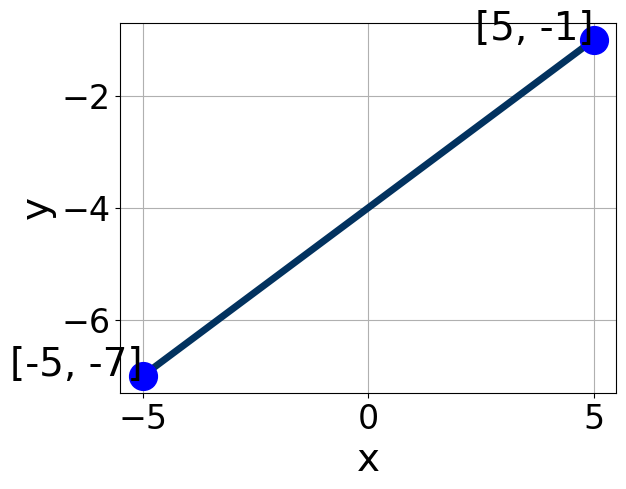
\includegraphics[width=0.5\textwidth]{../Figures/linearGraphToStandardB.png}
\end{center}
\begin{enumerate}[label=\Alph*.]
\item \( A \in [3, 12], \hspace{3mm} B \in [-7.5, -4.4], \text{ and } \hspace{3mm} C \in [20, 25] \)
\item \( A \in [-0.6, 0.4], \hspace{3mm} B \in [-3, -0.1], \text{ and } \hspace{3mm} C \in [3, 7] \)
\item \( A \in [-11, -2], \hspace{3mm} B \in [3.8, 7.8], \text{ and } \hspace{3mm} C \in [-20, -15] \)
\item \( A \in [3, 12], \hspace{3mm} B \in [3.8, 7.8], \text{ and } \hspace{3mm} C \in [-20, -15] \)
\item \( A \in [-0.6, 0.4], \hspace{3mm} B \in [-0.6, 1.4], \text{ and } \hspace{3mm} C \in [-13, 0] \)

\end{enumerate} }
\litem{
First, find the equation of the line containing the two points below. Then, write the equation in the form $ y=mx+b $ and choose the intervals that contain $m$ and $b$.\[ (9, -7) \text{ and } (-10, -3) \]\begin{enumerate}[label=\Alph*.]
\item \( m \in [-0.59, 0.04] \hspace*{3mm} b \in [6.5, 8.1] \)
\item \( m \in [-0.59, 0.04] \hspace*{3mm} b \in [4.7, 5.5] \)
\item \( m \in [-0.59, 0.04] \hspace*{3mm} b \in [-17.2, -14.8] \)
\item \( m \in [-0.59, 0.04] \hspace*{3mm} b \in [-5.5, -1.1] \)
\item \( m \in [0.07, 0.95] \hspace*{3mm} b \in [-2.3, 0.2] \)

\end{enumerate} }
\end{enumerate}

\end{document}